% 修士論文テンプレート

\documentclass[10pt]{jreport}

\usepackage{master_thesis}
\usepackage{./grad}
\usepackage[dvipdfmx]{graphicx}
\usepackage{here}
\usepackage{url}
\usepackage{bm}
\usepackage{amsmath}
\usepackage{comment}

% A4 : width 21cm, height 29.7cm
\usepackage[a4paper,textheight=21.7cm,top=3cm,left=2cm,right=2cm,headheight=15pt]{geometry}

\年度{2021}
\題目{VANETにおける車両位置とリンク状態を考慮した地理的
opportunistic routing}
\指導教官{野口 拓}
\学籍番号{6611200033-0}
\氏名{高橋 柊人}
\コース{計算機科学コース} %計算機科学コース or 人間情報科学コース


\begin{document}
% 表紙 %%%
\maketitle


\renewcommand{\thepage}{\roman{page}}
\setcounter{page}{1}
\addcontentsline{toc}{chapter}{内容梗概}
\chapter*{内容梗概}
本論文は,筆者が立命館大学情報理工学研究科において行った「VANETにおける車両位置とリンク状態を考慮した地理的
opportunistic routing」の成果をまとめたものである.

test


\newpage
\pagestyle{myheadings}
\renewcommand{\thepage}{\roman{page}}
%\setcounter{page}{1}
\addcontentsline{toc}{chapter}{目次}
%\setcounter{page}{1}
\tableofcontents


\newpage
\renewcommand{\thepage}{\arabic{page}}
\setcounter{page}{1}
\chapter{緒論}
\vspace{-5mm}

高速道路や一般道での無謀な運転や不注意運転によるほかのドライバへの危険が問題となっている. もし, これらの危険行為を行う車両の接近を遭遇する以前に知ることができれば, 多くの事故を減らすことができる可能性がある. 交通死亡事故の原因の中では, 規制速度を超過した場合の割合が31.6%\cite{1}と, 速度違反が死亡事故につながることがわかる. また, 交通事故死亡者数と取り締まり件数に注目すると, 取り締まりが増加すると死者数が減少するデータもある. これらのことから, 交通事故の死亡者数を減らすためには, より多くの速度超過の監視が求められる. 
 

そこで本論文では, VANETを用いたブロードキャスト数を最小限に抑えたVANETを用いた速度超過車両検出手法を提案する.速度超過車両の検出確率や,ブロードキャスト数を調査し,有効性を示す.

第2章では, VANETの概要を説明し, 既存方式について述べる. 第3章では, VANETを用いた速度推定法, ネットワークトラヒック量の削減を目的としたブロードキャスト制御アルゴリズムについて述べる. 第4章では, 評価方法について述べ, 本研究の評価方法を基に検証した結果をまとめる. 第5章は結論であり, 本研究の主な結果をまとめる. 



\chapter{VANET}
\vspace{-5mm}
\section{概要}
近年, 情報通信技術の発達により, 無線通信を用いて車両間または, 路車間で情報をやり取りすることによって交通事故や渋滞などの道路交通問題の解決を目指す高度道路交通システム(ITS:Inteligent Transport System)が注目を浴びている\cite{sample7}. ITSの代表的なサービスとして, 渋滞情報と連動した高度なナビゲーションシステム(VICS::Vehicle Information and Communication System)\cite{sample8}や, 自動料金収受システム(ETC:Electronic Toll Collection)\cite{sample9}などがあげられる. これらのサービスを支える技術として, 路車間通信と車両アドホックネットワーク(VANET)がある. 路車間通信は車両が路側機のインフラ設備との無線通信により情報のやりとりを行う. しかし, 路車間通信はインフラ設備の設置にかかる費用と, 設置場所が限定される可能性があるという問題が存在する. 一方, VANETは車両同士で通信を行うためインフラ設備の整備されていない不特定の場所でも通信を行うことが可能になる. VANETのアプリケーションとして, 渋滞回避情報の伝搬, 緊急車両情報の警告など, 安全運転支援に期待されている. 
\section{車車間通信}
車車間通信は車両と車両との間で無線通信を行い, 情報のやり取りを行うものである. 車車間通信を図2.1に示す. 車車間通信では, 端末同士(車両同士)で自律的にネットワークを構築し, 宛先に直接通信できない場合には間の車両が中継車両となり, マルチホップ通信を行う. 車車間通信のメリットは固定のインフラを必要とせず車両間のみで通信が可能になり, インフラが存在しない地点で通信が可能になることである. 
\section{路車間通信}
路車間通信は, 道路に設置された路側機(RSU:Road Side Unit)と車両で無線通信を行い 
様々な情報の交換を行うものである. 路車間通信を図2.1に示す.  路車間通信の代表的なサービスとしてVICS(Vehicle Information and Communication System)やETC(Electronic Toll Collection)がある. VICSは, 各道路に設置されたビーコンから道路交通情報を発信し, 車載のカーナビや高速道路の電子掲示板に高速道路の渋滞の情報, 区間を通過するための所要時間, 駐車場情報などを表示する「ナビゲーションシステム高度化」を目指したサービスである. ETCは高速道路の入り口に設置されている通信機と車載の通信機で無線通信を行い, 料金所に止まることなく, 自動でスムーズに料金の支払いができるシステムである. 料金所での一時停止が渋滞の原因の一つであったが, ETCの導入で渋滞を解消することができた. 




%図の入れ方
\begin{figure}[!ht]
\centering
\includegraphics[width=15cm]{figures/2_2.png}
\caption{車車間通信と路車間通信}
\end{figure}


\section{ルーチングプロトコル}
\label{RoutingProtocol}
VANETを都市環境で展開する場合, 高速な移動性, 不均一な車両密度, 樹木や建物による電波の遮断など様々な要件を考慮する必要がある. この様々な要件に対応するため, 多種多様なルーチングプロトコルが提案されている\cite{2}. 次節以降でそれぞれのルーチングプロトコルの特徴について述べる.

\subsection{Topology-based routing}
\label{Topology}
Topology-base routing\cite {3,4,5} は, ネットワークに存在するリンクに関する情報を使用して, パケット転送を行う方式である. Topology-based routingはProactive型とReactive型に分類できる. 前者は, ノード間で周期的な制御パケットの交換を行うことにより, 各ノードがすべての宛先ノードへの経路情報を常時保持する方式である. 後者は, 最初は経路情報は保持しておらず, 通信要求が生じてから, 制御パケットを交換し経路情報を作成する方式である. 前者と比較して後者は, 制御パケットのオーバヘッドを抑えられるというメリットがある. 
しかし, これらのTopology-based routingは, ノードが頻繁に移動するVANETにおいては, 経路情報を定期的に変更する必要がある.
したがって, 制御パケットのオーバーヘッドが増加するためVANETには適していない.

\subsection{Geographic routing}
\label{Geographic}
Geographic routing\cite{6,7,8,9,10,11,12,13,14,15} は, 隣接ノードの位置情報と宛先ノードの位置に基づいてパケット転送を行う方式である. このタイプのルーチングプロトコルは, Topology-based routingのように確立されたルートを維持する必要がない. したがってGeographic routingは制御パケットを使用する必要がないため, 少ないパケット数でトポロジーの変化に対応することができる. Greedy fowardingはGeographic routingにおいて有名な方式の一つである. Greedy fowardingは隣接ノードの中で最も宛先ノードに近いノードを中継ノードとして選択することで, ホップ数やオーバヘッドの削減を示している. しかし, 実際の都市環境では, 建物によるシャドウイングや距離による電波強度の低下によりパケットのドロップ率が高くなる可能性がある. 

\subsection{Opportunistic routing}
\label{Opportunistic}
上記のルーチングの問題点を解決できる可能性がある, Opportunistic routing\cite{16} が近年注目を集めている. Opportunistic routingと前述したルーチングプロトコルとの主な違いは固定経路を使用せず, 送信ノードが次の中継ノードを1つに決定しないことである(図\ref{fig:Gegraphic_opportunistic}). Opportunistic routingではブロードキャストの性質を利用し, 受信したノード同士が協調しパケットを再ブロードキャストするか否かを決定することでパケット到達率の向上とオーバーヘッドの削減を果たしている. 

Opportunistic routingは主に次の4ステップで構成されている.

\begin{itemize}
	\item 中継候補ノードセット(RCS) の選択
	\item RCSの優先順位を決定
	\item RCSへのブロードキャスト
	\item 優先順位に応じた再ブロードキャストをするか否かの決定(RCS同士の協調)
\end{itemize}

図\ref{fig:Basic1}, \ref{fig:Basic2}にOpportunistic routingの基本モデルを示す.
$N_{s}$が送信ノード, $N_{d}$が宛先ノードである. 送信ノード$N_{s}$はRCSとして$N_{1}$ ~ $N_{n}$を選択する. 次に送信ノードは選択したRCSそれぞれに優先順位を指定してパケットをブロードキャストする. 受信した$N_{1}$ ~ $N_{n}$のノードはそれぞれ自身の優先順位を確認し, 中継タイマー(待ち時間)を設定する. 中継タイマーは優先順位が高いノードほど早くタイムアウトするように設定し, タイマーが切れたノードから再ブロードキャストを行う. 自身の中継タイマーが切れる前に自身より優先順位が高いノードの再ブロードキャストを受信した場合, 自身の再ブロードキャストをキャンセルし, 冗長なパケットの増加を防ぐ.
 

\begin{figure}[!ht]
	\centering
	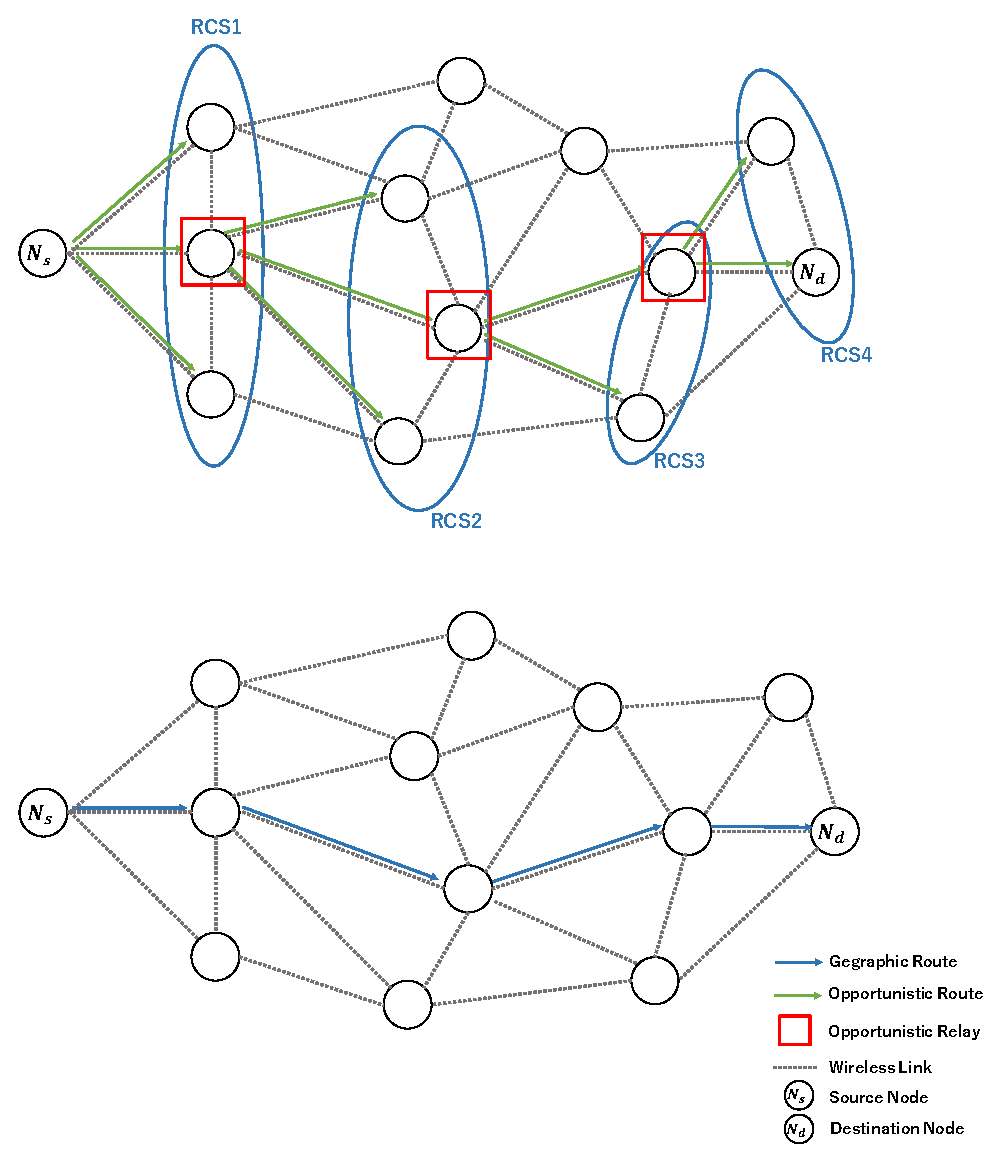
\includegraphics[width=150mm]{figures/difference_geographic_opportunistic.eps}
	\caption{Geographic routingとOpportunistic routing}
	\label{fig:Gegraphic_opportunistic}
\end{figure}

\begin{figure}[!ht]
	\centering
	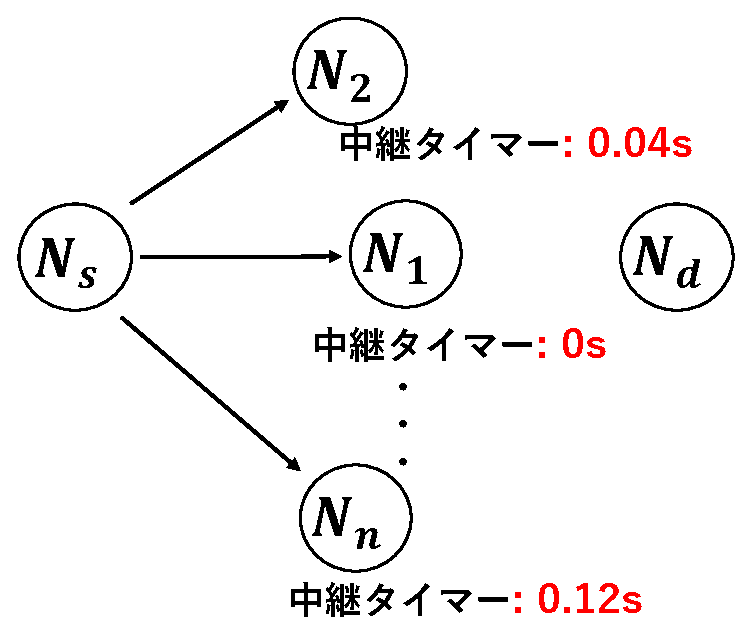
\includegraphics[width=90mm]{figures/basic-opportunity1.eps}
	\caption{Opportunistic routingの基本モデル1}
	\label{fig:Basic1}
\end{figure}

\begin{figure}[!ht]
	\centering
	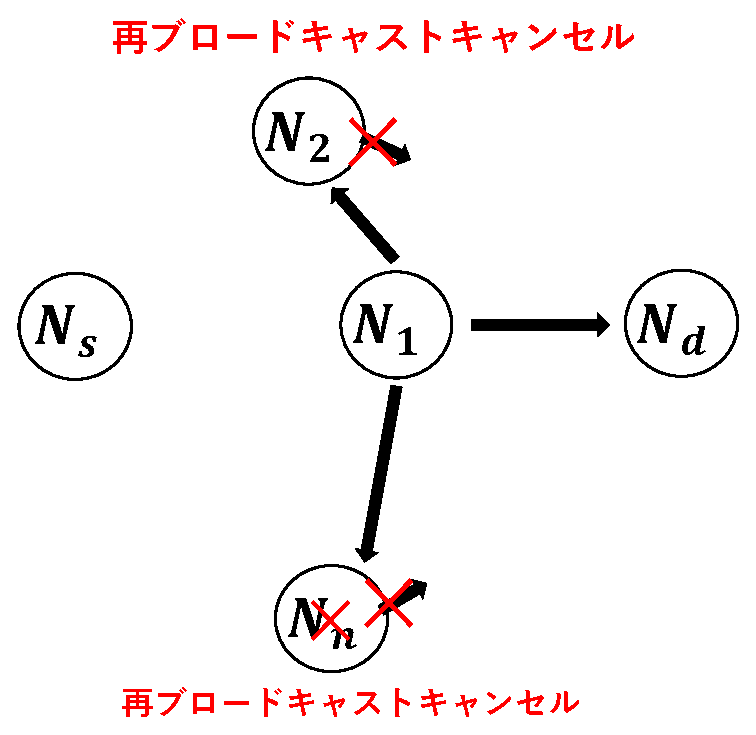
\includegraphics[width=90mm]{figures/basic-opportunity2.eps}
	\caption{Opportunistic routingの基本モデル2}
	\label{fig:Basic2}
\end{figure}

これらのことから, Opportunistic routingにおいて, 優先順位決定アルゴリズムが通信性能に直接影響を及ぼすことがわかる.

代表的なOpportunistic routingとしてOpportunistic multi-hop routing fo wireless networks(EXOR) \cite{16}が提案されている. これは, RCSの優先順位を決定するメトリックとして, Expected transmission cost(ETX) \cite{21}を用いている. しかし, ETX値はVANETの性質であるノードのランダムで高速なモビリティを考慮していないという問題がある.

そこで, 新たにVANETに適したETX値を考案したLink state aware geographic opportunistic routing protocol(LSGO) \cite{18}が提案された. LSGOでは, VANET用に最適化されたETX値をRCSの優先順位を決定するメトリックとして使用し, パケット到達率の向上, エンドツーエンド遅延の減少を実現している. また, Collision-aware opportunistic routing protocol (SCAOR) \cite{22}では, パケットの衝突でネットワークパフォーマンスを低下させる問題を防ぐために, ノード密度パラメータをRCSの優先順位を決定するメトリックとして追加した. その結果, 高速道路においてEXORやLSGOに比べ通信性能が向上することを示している. Hybrid opportunistic and position-based routing  protocol (OPBR) \cite{23}では, パケットがRCSに到達しない場合, 遅延が増加するという問題を解決するために, 隣接ノードの位置情報からリンクの切断を推測した. この結果パケット到達率の向上, エンドツーエンド遅延の減少を示している.

しかし, 既存のopportunistic routingの多くは, 都市環境を想定して考案されているが, 性能評価で建物によるシャドウイングの影響が考慮されておらず, 通信性能を過大評価している可能性がある. また, これによりシャドウイングの影響を考慮したルーティングプロトコルが設計されていない可能性がある. 

そこで, 本研究では, 既存opportunistic routingであるLSGOをネットワークシミュレータNS-3\cite{19}のシャドウイングモデルであるObstacle Shadowing Model\cite{20}を用いて評価し, 建物によるシャドウイングが起こる場合と起こらない場合の通信性能を検証し, 問題点を明らかにする.





\subsection{Geocast routing}
Topology-base routing\cite {3,4,5} は, 

\section{Local optimum problem}
\label{local_optimum_problem}
\ref{Geographic}節で紹介したGeographic routingの既存研究では, 各送信ノードは自分より宛先ノードに近い隣接ノードの中から中継ノードとして最適なノードを1つ選択する. 同様に\ref{Opportunistic}節で紹介した多くのVANET用に設計されたOpportunistic routingにおいても, 各送信ノードは自分より宛先ノードに近い隣接ノードの中からCRSを選択する. しかし, 時には自分より宛先ノードに近い隣接ノードが存在しない場合が発生する. この問題をLocal optimum problem\cite{6}と呼ぶ. Local optimum problemは, 図\ref{fig:Local_optimum}のように建物による電波の遮断が起きやすい都市環境では発生確率が上昇する. したがって, 特にVANETにおいて自分より宛先ノードに近い隣接ノードから中継ノードを選択するタイプのルーティングでは, この問題を防ぐアプローチと発生した場合の対処法(recovery strategy) の考案が必用である.

\begin{figure}[!ht]
	\centering
	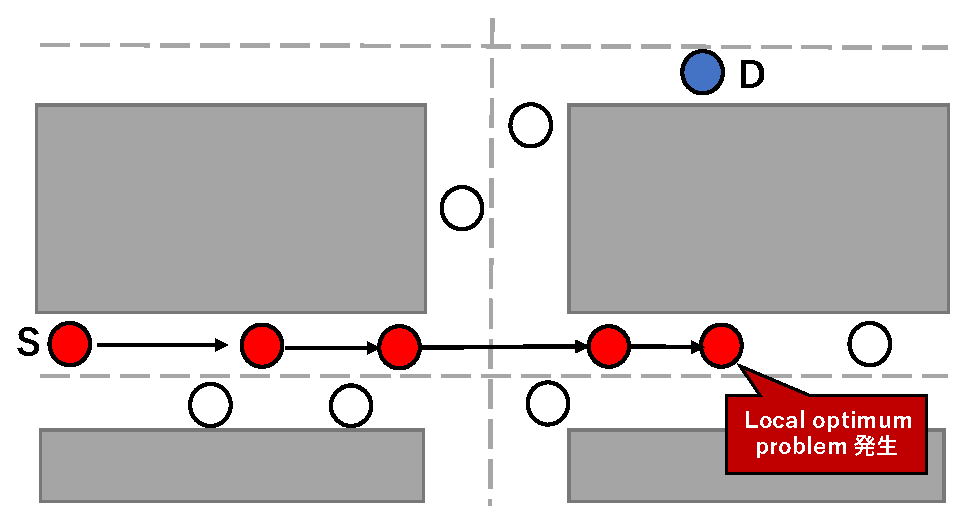
\includegraphics[width=130mm]{figures/Local_optimum_problem.eps}
	\caption{Local optimum problem}
	\label{fig:Local_optimum}
\end{figure}

\section{Recovery strategy}
前節で説明したLocal optimum problemがルーチング中に発生した場合, これに対処する中継戦略が必要となる. これをRecovery strategy\cite{28}と呼ぶ. revovery strategyの基本モデルを図\ref{fig:Recovery}に示す. $N_{1}$でLocal optimum problemが発生する. 次に$N_{1}$は, 自身の位置情報をパケットに加えrecovery strategyを開始する. recovery strategyは, Local optimum problemが発生したノード($N_{1}$)の位置より宛先に近いノードにパケットが到達するまで繰り返される. $N_{2}$までパケットが到達した場合$N_{2}$は$N_{1}$よりも宛先に近いため, 元の中継を開始する. 
  

\begin{figure}[!ht]
	\centering
	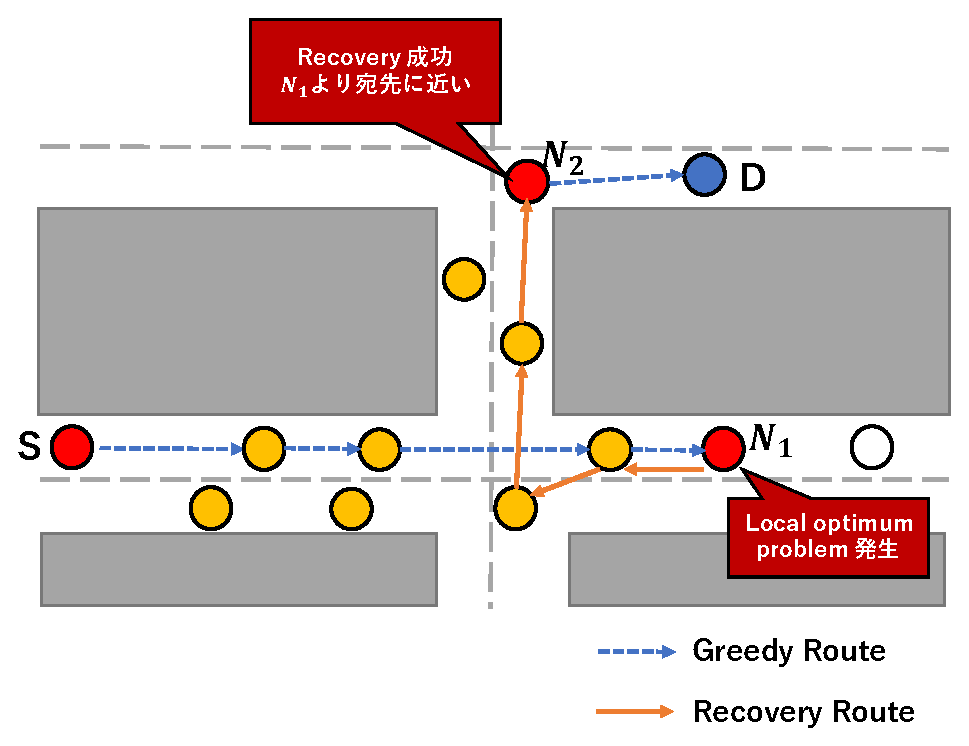
\includegraphics[width=130mm]{figures/basic-recovery.eps}
	\caption{Recovery strategy}
	\label{fig:Recovery}
\end{figure}

代表的なrecovery strategyとしてGreedy perimeter stateless routing(GPSR) \cite{6}の $perimeter forwarding$
と呼ばれるrecovery strategyが提案されている. 

\addcontentsline{toc}{chapter}{謝辞}
\chapter*{謝辞}
\sloppy
本論文では筆者が立命館大学情報理工学部情報コミュニケーション学科におい
て行なった「VANETを用いた速度超過車両検出のためのブロードキャスト制御法」の成果をまとめたものである.

本研究を遂行するにあたり,全過程を通じて懇切丁寧なる御指導,御鞭撻を賜わっ
た,立命館大学情報理工学部野口~拓教授に深甚なる感謝の意を表す.

立命館大学情報理工学部において,御指導,御教授を賜わった立命館大学情報理工学部Alberto Gallegos Ramonet特任助教, 前田~忠彦教授, 山本~寛准教授, 西村~俊和准教授, 瀧本~栄二助教を始め,各教員の方々に衷心より御礼申し上げる.

%本研究を遂行するにあたり,終始一貫して直接御指導戴いたネットワークシステム研究室の野口~拓講師に深甚なる感謝の意を表す.

ネットワークシステム研究室の諸兄には,日頃より多くの御助言,御協力戴き,種々の面でお世話になった.ここに深謝申し上げる.

ここに記して,以上の方々に深甚なる感謝の意を捧げる.

\addcontentsline{toc}{chapter}{参考文献}

%\newpage

\bibliographystyle{IEEEtran}
\bibliography{shuto}


\end{document}
